% !TEX root = ../agglo_clust_review.tex

\captionsetup[subfigure]{justification=centering, singlelinecheck=off}
\begin{figure*}
\centering
    \begin{subfigure}[t]{0.49 \textwidth}
        \centering
        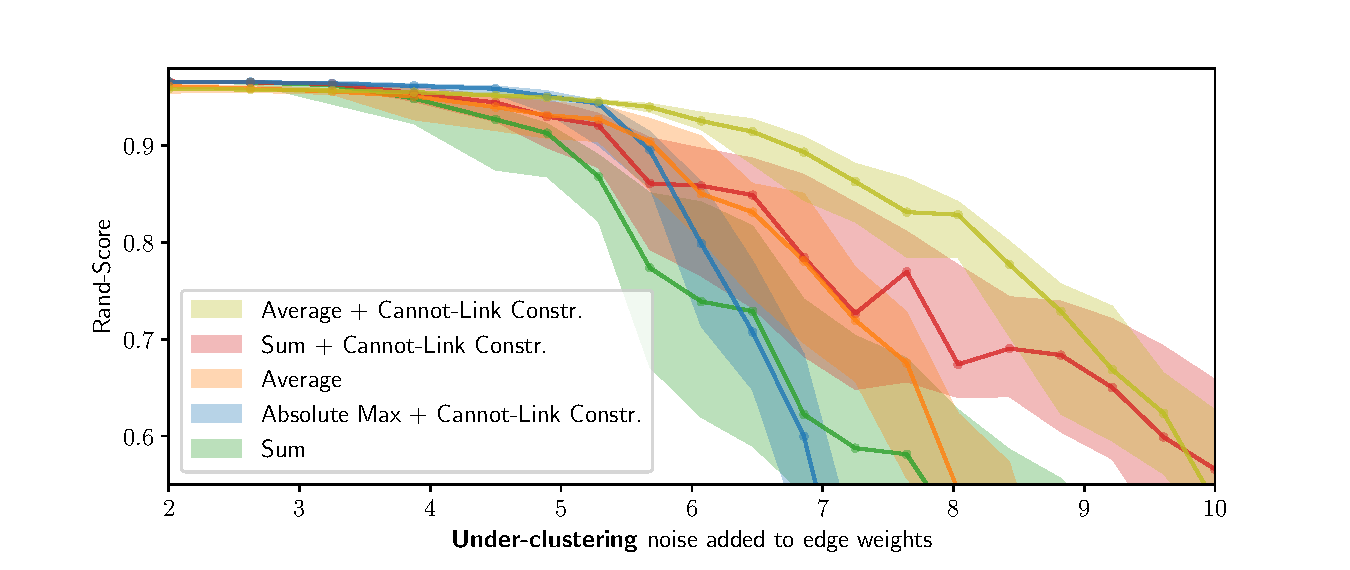
\includegraphics[width=\textwidth,trim=0.55in 0.1in 0.65in 0.45in,clip]{./figs/noise_plots/under_segment_plots_0.pdf}
    \end{subfigure} \hfill
    \begin{subfigure}[t]{0.49 \textwidth}
        \centering
        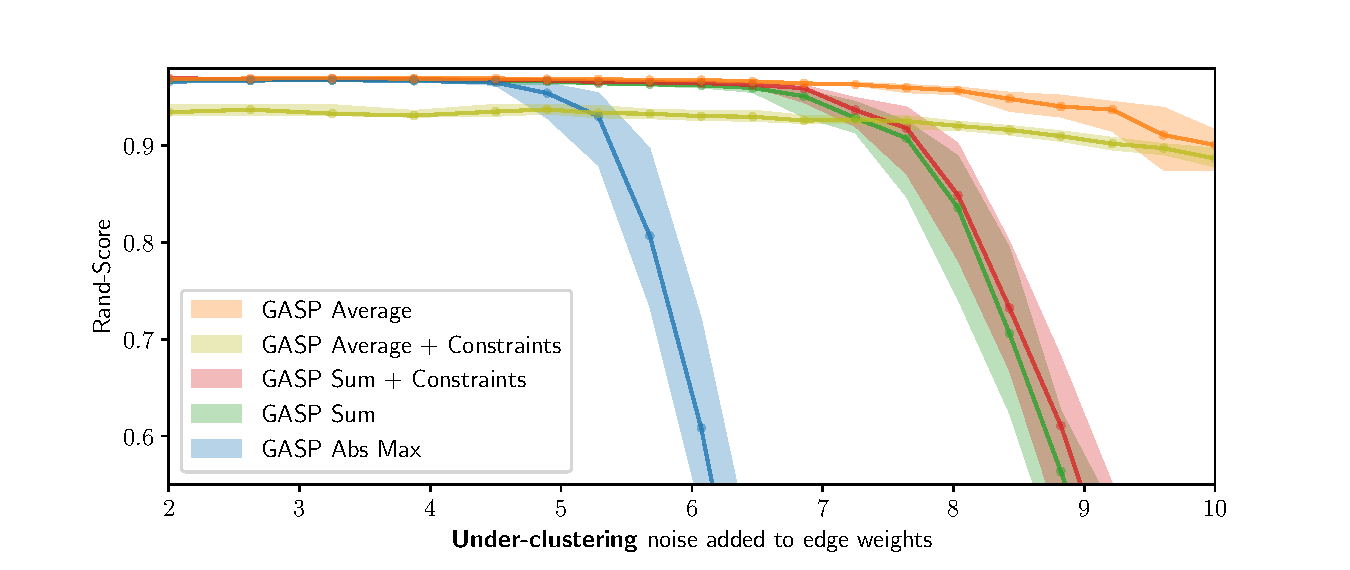
\includegraphics[width=\textwidth,trim=0.53in 0.1in 0.65in 0.45in,clip]{./figs/noise_plots/under_segment_plots_1.pdf}
    \end{subfigure}

        \begin{subfigure}[t]{0.49 \textwidth}
        \centering
        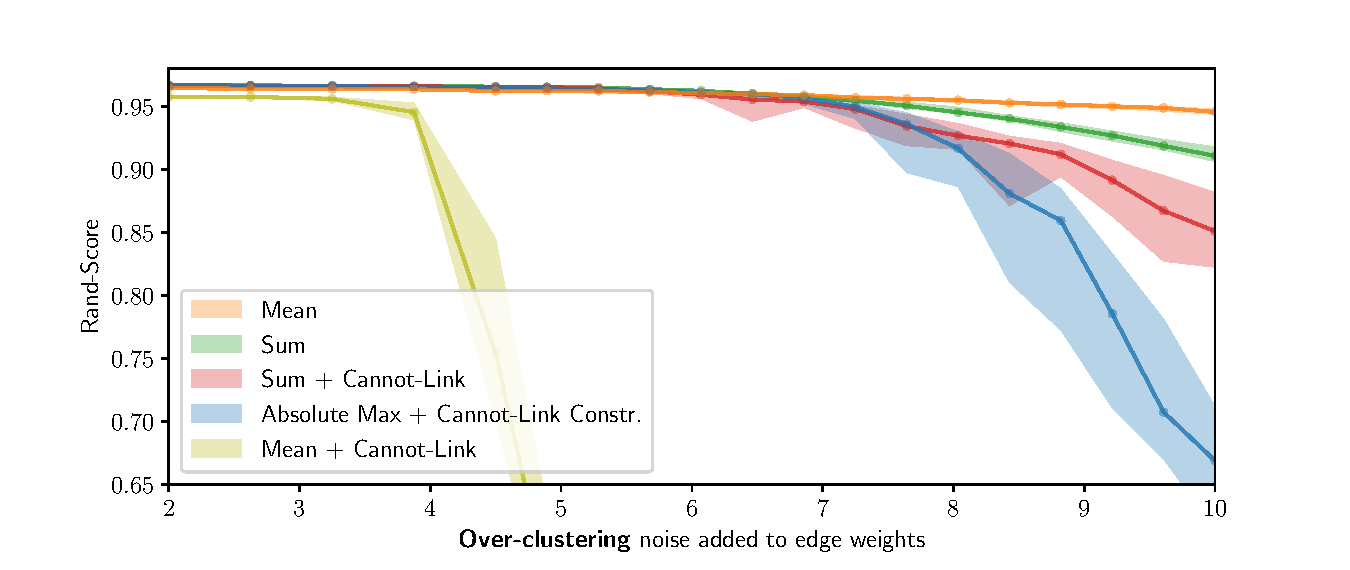
\includegraphics[width=\textwidth,trim=0.53in 0.1in 0.65in 0.45in,clip]{./figs/noise_plots/over_segment_plots_0.pdf}
        \caption{No long-range predictions: $p_{\mathrm{long}}=0$} \label{fig:merge_noise_only_direct}
    \end{subfigure} \hfill
    \begin{subfigure}[t]{0.49 \textwidth}
        \centering
        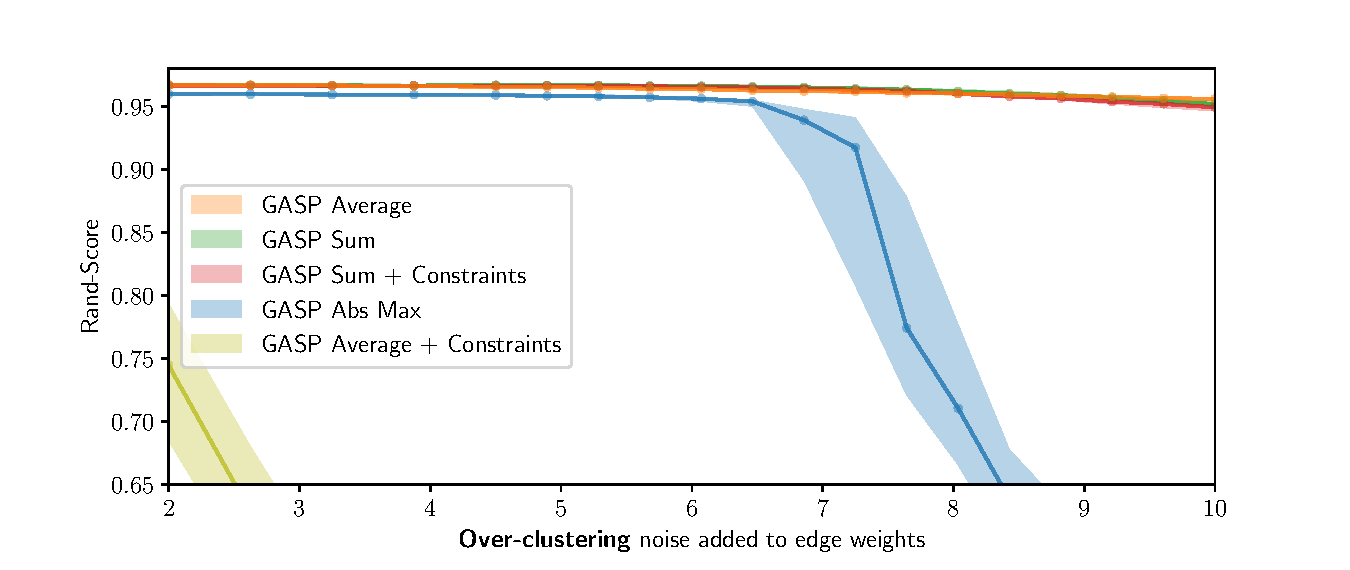
\includegraphics[width=\textwidth,trim=0.53in 0.1in 0.65in 0.45in,clip]{./figs/noise_plots/over_segment_plots_1.pdf}
        \caption{With long-range predictions: $p_{\mathrm{long}}=0.1$} \label{fig:merge_noise_with_long_range}
    \end{subfigure}
\caption{\algname{} sensitivity to noise: \emph{Average} linkage proved to be the most robust. Performances are given by Rand-Score (higher is better) depending on the amount of noise added to the CNN predictions. Solid lines represent median values over 30 experiments. Values between the 25th and the 75th percentile are shown in shaded areas. The two sets of experiments using under- and over-clustering noise are summarized in the plots at the top and at the bottom, respectively (see Appendix \ref{sec:appendix_noise_gen} for more details). For each experiment, some of the long-range CNN predictions were randomly selected with probability $p_{\mathrm{long}}$ and added as long-range edges to the pixel grid-graph. Experiments are performed on a crop of CREMI training sample B.
}\label{fig:noise_plots}
\end{figure*}
\begin{figure*}[t]
        \centering
\begin{minipage}[t]{0.31\textwidth}
    \centering
    \scriptsize
        \begin{tabular}[t]{l|c}
          & \makecell{CREMI-Score \\(lower is better)} \\ \midrule 
\textbf{\algname{}} \textbf{Average}& \textbf{0.226}  \\
\algname{} Sum + Constraints \cite{levinkov2017comparative} & 0.282 \\
\algname{} Abs. Max. \cite{wolf2018mutex} & 0.322 \\
\algname{} Max. + Constraints & 0.324 \\
\algname{} Sum \cite{keuper2015efficient} & 0.334 \\
\algname{} Average + Constraints & 0.563 \\
THRESH & 1.521 \\ 
        \end{tabular}
    \captionof{table}{CREMI-Scores achieved by different linkage criteria and thresholding. All methods use the affinity predictions from our CNN as input. Scores are averages over the three CREMI training datasets.}
    \label{tab:results_cremi_train}
\end{minipage}\hfill
\begin{minipage}[t]{0.3\textwidth}
    \centering
    \scriptsize
        \begin{tabular}[t]{l|c}
         & \makecell{CREMI-Score \\(lower is better)}  \\ \midrule
Our CNN + DTWS + LMC &  0.221\\
PNI CNN \cite{lee2017superhuman} & 0.228 \\
\textbf{Our CNN + \algname{} Average} & \textbf{0.241} \\
MALA CNN + MC \cite{funke2018large} & 0.276 \\
CRU-Net \cite{zeng2017deepem3d} & 0.566  \\
LFC \cite{parag2017anisotropic} & 0.616  \\
        \end{tabular}
        \vspace*{4.5em}
    \captionof{table}{Current leading entries  in the CREMI challenge leaderboard \cite{cremiChallenge} (May 2019). The scores are averages of the three test datasets.}
    \label{tab:results_cremi_test}
\end{minipage}\hfill
\begin{minipage}[t]{0.32\textwidth}
\centering
    \scriptsize
    \vspace*{-1.5em}
\begin{tabular}[t]{l|cc}
            & AP  & AP 50\% \\ 
        Method & \multicolumn{2}{c}{(higher is better)} \\ \midrule
           Panoptic-DeepLab \cite{cheng2019panopticdeeplab} & 34.6 & 57.3 \\
           UPSNet \cite{xiong2019upsnet} $\dagger$ & 33.0 & 59.6 \\
           SSAP \cite{Gao_2019_ICCV} & 32.7 & 51.8 \\
           PANet \cite{liu2018path} $\dagger$ & 31.8 & 57.1 \\
           \textbf{GMIS Model + \algname{} Average} & \textbf{28.3} & \textbf{47.0} \\ 
           JOSECB \cite{neven2019instance} & 27.7 & 50.9 \\
           \textbf{GMIS Model} \cite{liu2018affinity} & \textbf{27.3} & \textbf{45.6} \\
           Mask R-CNN \cite{he2017mask} $\dagger$ & 26.2 & 49.9 \\
           SGN \cite{liu2017sgn} & 25.0 & 44.9 \\
           % DIN \cite{arnab2017pixelwise} & 20.0 & 38.8 \\
           DWT \cite{bai2017deep} & 19.4 & 35.3 \\
           InstanceCut \cite{kirillov2017instancecut} & 13.0 & 27.9 \\
        \end{tabular}
    % \caption{CityScapes \emph{test} set}
    \vspace*{0.7em}
    \captionof{table}{Average Precision scores on CityScapes test. Methods marked with $\dagger$ are \emph{proposal-based}.}\label{tab:results_cityscapes}
    \label{tab:results_cityscapes_test}
\end{minipage}
\end{figure*}

\captionsetup[subtable]{labelformat=simple, labelsep=space, justification=centering, singlelinecheck=off}
\renewcommand*{\thesubtable}{(\alph{subtable})}
\begin{figure*}[t]
\begin{minipage}{0.65 \textwidth}
\centering
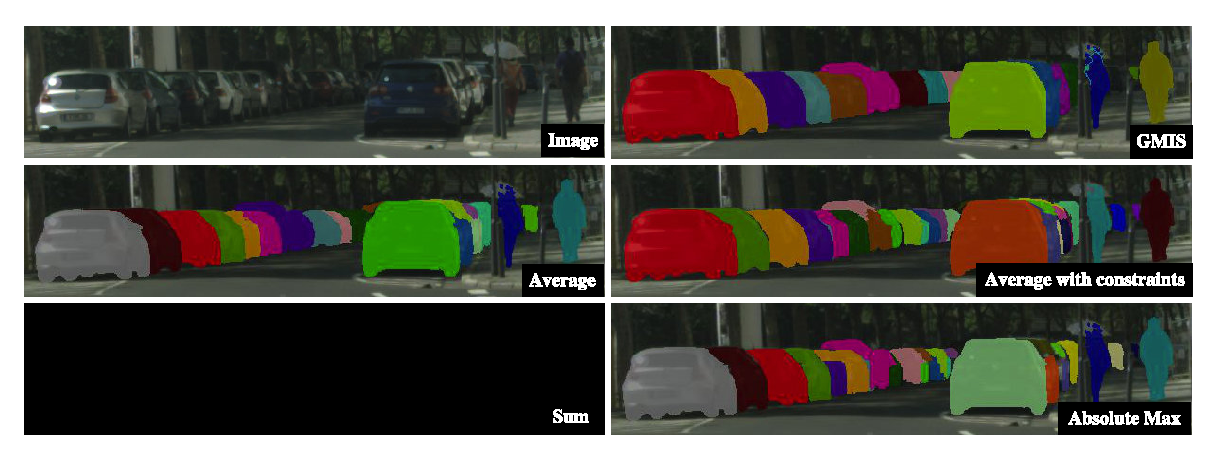
\includegraphics[width=\textwidth]{./figs/cityscapes_compare_5.eps} % left bottom right top
\caption{Visual results given by different \algname{} linkage criteria on a crop of a CityScapes image}\label{fig:cityscapes}
\end{minipage}\hfill
\begin{minipage}{0.3 \textwidth}
    \centering
    \small
        \begin{tabular}[t]{l|cc}
             Agglomeration type & AP \\ \midrule
            % PANet \cite{liu2018path} & - & \textbf{36.5} \\
            % Mask R-CNN \cite{he2017mask} & - & 31.5 \\ \hline
              \algname{} Average& 34.3 \\
              \algname{} Average + Constraints & 33.9 \\
             MultiStepHAC \cite{liu2018affinity} & 33.0 \\
              \algname{} Abs. Max. \cite{wolf2018mutex}  & 32.1 \\
              \algname{} Sum + Constraints  \cite{levinkov2017comparative} & 31.9  \\
              \algname{} Sum \cite{keuper2015efficient} & 31.3 \\
        \end{tabular}
    \vspace*{0.6em}
    \caption{Average Precision scores on CityScapes \emph{val} achieved by the GMIS Model \cite{liu2018affinity} and different graph agglomeration methods.}
    \label{tab:results_cityscapes_val}
\end{minipage}
\end{figure*}

\subsection{Results and discussion}\label{sec:results}
\textbf{Comparison of linkage criteria} Table \ref{tab:results_cremi_train} shows how the agglomerative algorithms derived from our framework compare to each other. For a simple baseline, we also include a segmentation produced by thresholding the affinity predictions (THRESH).
\algname{} with \emph{Average} linkage, representing one of the new algorithms derived from our generalized framework, significantly outperformed all other previously proposed agglomerative methods like GAEC (\algname{} Sum) \cite{keuper2015efficient}, Greedy Fixation (\algname{} Sum + Constraints) \cite{levinkov2017comparative} or Mutex Watershed (\algname{} Abs. Max.) \cite{wolf2018mutex}. The competitive performance of this simple parameter-free algorithm is also reported in Table \ref{tab:results_cremi_test}, showing the current leader-board of the challenge: all entries, apart from \algname{}, employ superpixel-based post-processing pipelines, several of which rely on the lifted multicut formulation of \cite{beier2017multicut} that uses several random forests to predict graph edge weights, relying not only on information derived from affinity maps but also raw data and shape information.
Note that the test volumes contain several imaging artifacts that make segmentation particularly challenging and might profit from more robust edge statistics of super-pixel based approaches.
On the other hand, the fact that our algorithm can operate on pixels directly removes the parameter tuning necessary to obtain good super-pixels and can also avoid errors that result from wrong superpixels that cannot be fixed during later agglomeration.
In Appendix \ref{sec:appendix_exps_full_cremi}, we provide more details about how we scaled up \algname{} to the full datasets. Appendix Table \ref{tab:extended_results_cremi} lists the performances and the run-times for all tested \algname{} linkage.





\textbf{Noise experiments }  Additionally, we conduct a set of experiments where the CNN predictions are perturbed by structured noise, in order to highlight the properties of each \algname{} variant and perform an in-depth comparison that is as quantitative as possible. Appendix \ref{sec:appendix_noise_gen} introduces the type of spatially correlated noise that allowed us to perturb the CNN outputs by introducing simulated additional artifacts like missing or false positive boundary evidence. 
Fig. \ref{fig:noise_plots} summarizes our 12000 noise experiments: we focus on the best performing linkage criteria, i.e. \emph{Average}, \emph{Sum} and \emph{Abs Max}, and test them with different amount of noise. 
In these experiments, we also want to assess how beneficial it is to use long-range CNN predictions in the agglomeration. Thus, we perform a set of simulations without adding long-range connections to the grid-graph and another set where we introduce them with a 10\% probability\footnote{We also performed experiments adding all the long-range predictions given by the CNN model, but we did not note major differences when using only 10\% of them. Adding this fraction is usually sufficient to improve the scores.}.

\textbf{Average and Abs Max linkage } Our findings confirm that \algname{} with \emph{Average} linkage criterion represents the most robust algorithm tested and the one that benefits the most from using the long-range CNN predictions. On the other hand, it is not a surprise that the \emph{Abs Max} statistic proposed by \cite{wolf2018mutex} is less robust to noise than the \emph{Average} linkage, but, as we show in the Appendix Table \ref{tab:extended_results_cremi}, \emph{Abs Max} represents a valid and considerably faster option. 
Adding long-range connections to the graph is generally helpful, but when many of them carry repulsive weights, then \algname{} with cannot-link constraints shows a clear tendency to over-cluster.    

\textbf{Sum linkage } 
All our experiments show that \algname{} with \emph{Sum} linkage is the algorithm with the highest tendency to under-cluster and incorrectly merge segments (see Fig. \ref{fig:cremi_comparison} for an example). This property is related to the empirical observation that a \emph{Sum} statistic tends to grow clusters one after the other, as shown in Fig. \ref{fig:intro_figure} by the quite unique agglomeration order of the \emph{Sum} statistic. An intuitive explanation of this fact is the following: initially, most of the intra-cluster nodes present similar attractive interactions between each others; when the two nodes sharing the most attractive interaction are merged, there is a high chance that they both share an attractive interaction with a common neighboring node, so the new interaction with this common neighbor will be immediately assigned to a high priority in the agglomeration, given by the sum of two high weights; this usually starts a ``chain reaction'', where only a single cluster is agglomerated at the beginning. On the other hand, as we also see in Fig. \ref{fig:intro_figure}, other linkage criteria like \emph{Average} or \emph{Abs Max} grow clusters of similar sizes in parallel and accumulate in this way much more reliable inter-cluster statistics.





